\begin{frame}
  \frametitle{System}
  \begin{itemize}
    \item Homogeneous base stations, mmWave, downlink transmission, OFDMA, multiple-input eMBB and single-input URLLC users.
    \item Saturated eMBB traffic \cite{S05}: Each eMBB user has \highlight{infinite} amount of data to be served.
    \item Strict URLLC constraint: Each URLLC has an amount of data required to be served within a minislot.
    \item The system aims to maximize eMBB total average rate and fairness while satisfying URLLC demands.
  \end{itemize}
\end{frame}

\section{Issues and Solutions}
\begin{frame}
  \frametitle{Multicell}
  \begin{figure}
    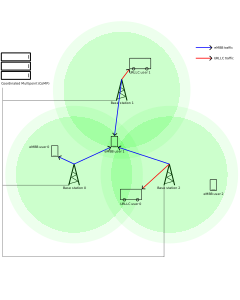
\includegraphics[width=0.5\textwidth]{model_multicell}
    \caption{Multicell model}
  \end{figure}
\end{frame}

\subsection{Spectrum Inefficiency}
\begin{frame}
  \frametitle{Spectrum Inefficiency}
  \begin{itemize}
    \item Dedicated URLLC bandwidth wastes spectral resources significantly in multicell systems.
      \begin{itemize}
        \item If $2$ subchannels of each base station are dedicated to URLLC traffic, then we would have $6$ subchannels sitting \highlight{idle for most of the time} in the aforementioned scenario.
      \end{itemize}
  \end{itemize}
\end{frame}

\begin{frame}
  \begin{itemize}
    \item This problem can be addressed by leveraging URLLC superposition/puncturing scheme. % TODO citations
    \item URLLC superposition scheme employs 5G NOMA SIC, whose performance equals to puncturing when the considered eMBB and URLLC users have the same channel gain. % TODO citations and example
    \item URLLC puncturing scheme is discussed here.
  \end{itemize}
\end{frame}

\begin{frame}
  \begin{figure}
    \includegraphics[width=1.05\textwidth]{framework_singlecell}
    \caption{Singlecell framework}
  \end{figure}
\end{frame}
